\section{Iluminación Global de Vóxeles} % (fold)
\label{sec:iluminacion_global_de_voxeles_impl}
En la sección anterior se expone el cálculo de iluminación indirecta de solo un rebote. Si se observa el Código \ref{Trace7} los únicos datos necesarios para este cálculo con solo el componente difuso son: albedo, normal, posición e iluminación directa.

Todos estos datos se encuentran disponibles en nuestra representación en vóxeles. La iluminación directa en vóxeles se obtiene luego del proceso de sombreado de vóxeles, mientras que albedo y normal son volúmenes producto del proceso de voxelización. La posición puede ser fácilmente proyectada utilizando la función \emph{VoxelToWorld} vista en el Código \ref{SpaceTransform}.

Nuestra implementación realiza iluminación global de solo el componente difuso sobre los vóxeles utilizando \emph{compute shaders}. El algoritmo de trazado es exactamente el mismo al expuesto en la sección anterior. La única diferencia es que este proceso se realiza por vóxel en vez de por píxel. El Código \ref{VoxelGI} expone este proceso:
\\
\begin{lstlisting}[caption={Calculo de iluminación global sobre vóxeles.}, label=VoxelGI]
// volúmenes de la representación en vóxeles
layout(binding = 0, rgba8) uniform image3D voxelComposite;
layout(binding = 1, rgba8) uniform sampler3D voxelAlbedo;
layout(binding = 2, rgba8) uniform sampler3D voxelNormal;
layout(binding = 3) uniform sampler3D voxelTexMipmap[6];
(*@\centerline{\raisebox{-1pt}[0pt][0pt]{$\vdots$}}@*)
void main()
{
    if(gl_GlobalInvocationID.x >= volumeDimension ||
        gl_GlobalInvocationID.y >= volumeDimension ||
        gl_GlobalInvocationID.z >= volumeDimension) return;

    ivec3 writePos = ivec3(gl_GlobalInvocationID);
    vec4 albedo = texelFetch(voxelAlbedo, writePos, 0);

    if(albedo.a < EPSILON) { return; }

    vec4 directLight = imageLoad(voxelComposite, writePos);
    // normal promedio del proceso de voxelización
    vec3 normal = texelFetch(voxelNormal, writePos, 0).xyz;
    // vector normal esta almacenado en formato 0->1, se convierte a -1->1
    normal = normalize(DecodeNormal(normal));
    // calcular el primer rebote de luz sobre el vóxel
    vec3 position = VoxelToWorld(writePos);
    vec4 indirectLighting = CalculateIndirectLighting(position, normal);
    // multiplicación por el albedo producto de la voxelización
    indirectLighting *= albedo;
    // composición luz directa + luz indirecta
    vec4 radiance = directLight + indirectLighting;
    radiance.a = directLight.a;
    // almacenar en la textura base de radiancia
    imageStore(voxelComposite, writePos, radiance);
}
\end{lstlisting}

El método \emph{CalculateIndirectLighting} es el mismo visto en la sección anterior, igualmente el trazado de conos pero sin oclusión ambiental. La textura \emph{voxelComposite} es la textura resultante del sombreado de vóxeles (Figura \ref{fig:hierarchy_impl}). Una vez terminado el cálculo de iluminación global sobre los vóxeles debe volver a realizarse el proceso de filtrado anisótropo descrito en la sección \ref{sub:voxeles_anisotropos}. Almacenar la iluminación global producto del primer rebote sobre los vóxeles nos permite aproximar el segundo rebote durante el proceso de trazado de conos de la sección anterior. En la Figura \ref{fig:vgi_scenes} se puede observar la escena voxelizada con iluminación global de vóxeles.
\begin{figure}[H]
	\centering
	\begin{subfigure}[t]{0.35\textwidth}
		\centering
		\captionsetup{justification=centering}
		\caption*{Solo iluminación directa.}
		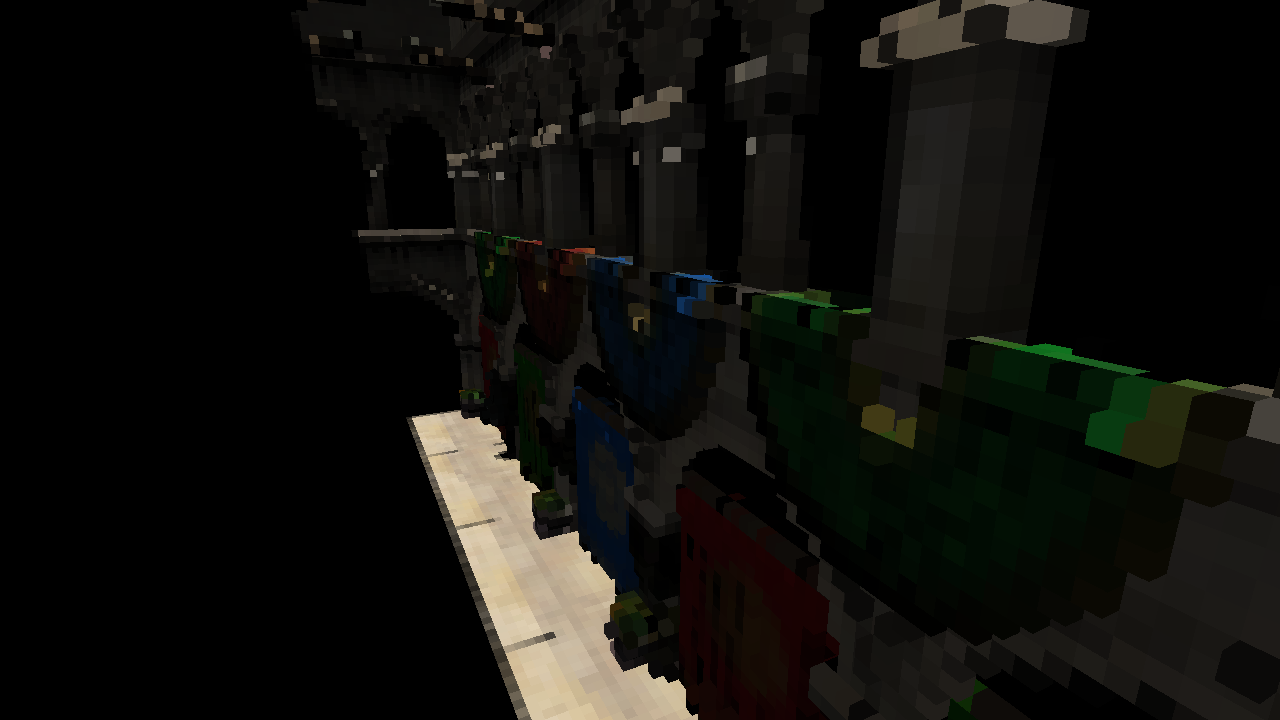
\includegraphics[width=\linewidth]{media/voxel_direct.png}
	\end{subfigure}%
	\hspace{0.05\textwidth}
	\begin{subfigure}[t]{0.35\textwidth}
		\centering
		\captionsetup{justification=centering}
		\caption*{Con iluminación indirecta.}
		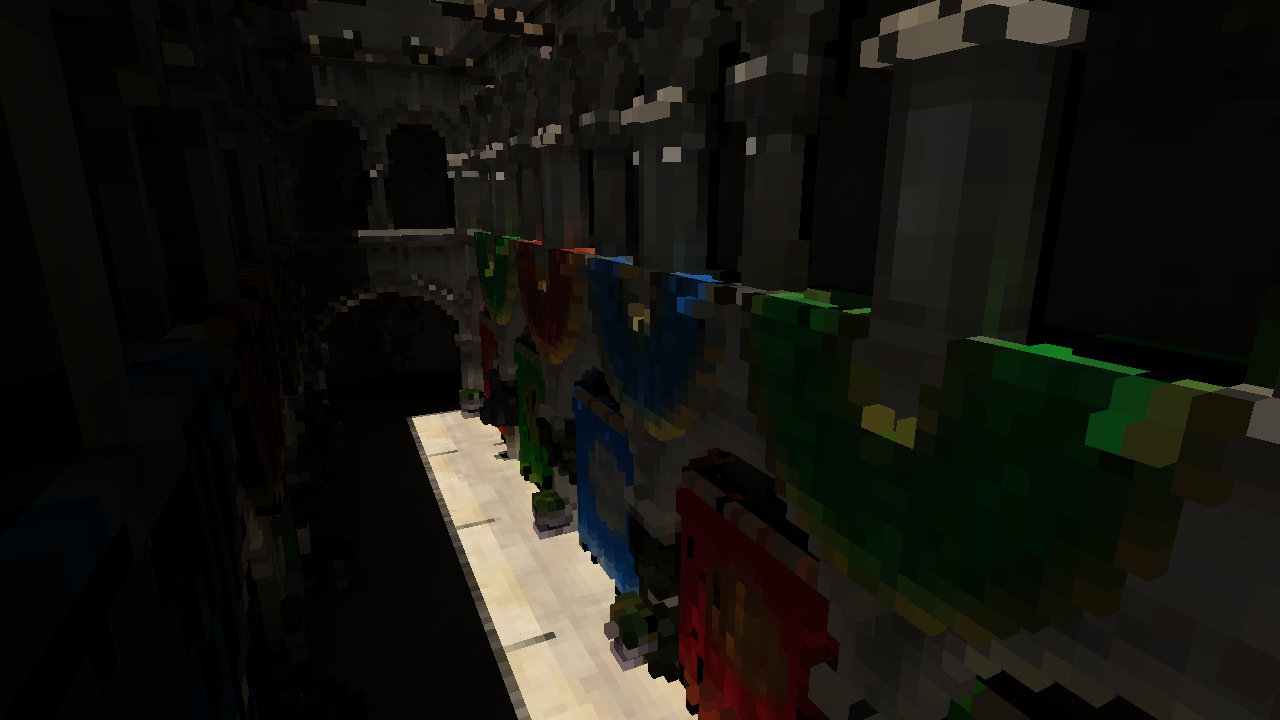
\includegraphics[width=\linewidth]{media/voxel_gi.png}
	\end{subfigure}%
	\par\smallskip
	\begin{subfigure}[t]{0.35\textwidth}
		\centering
		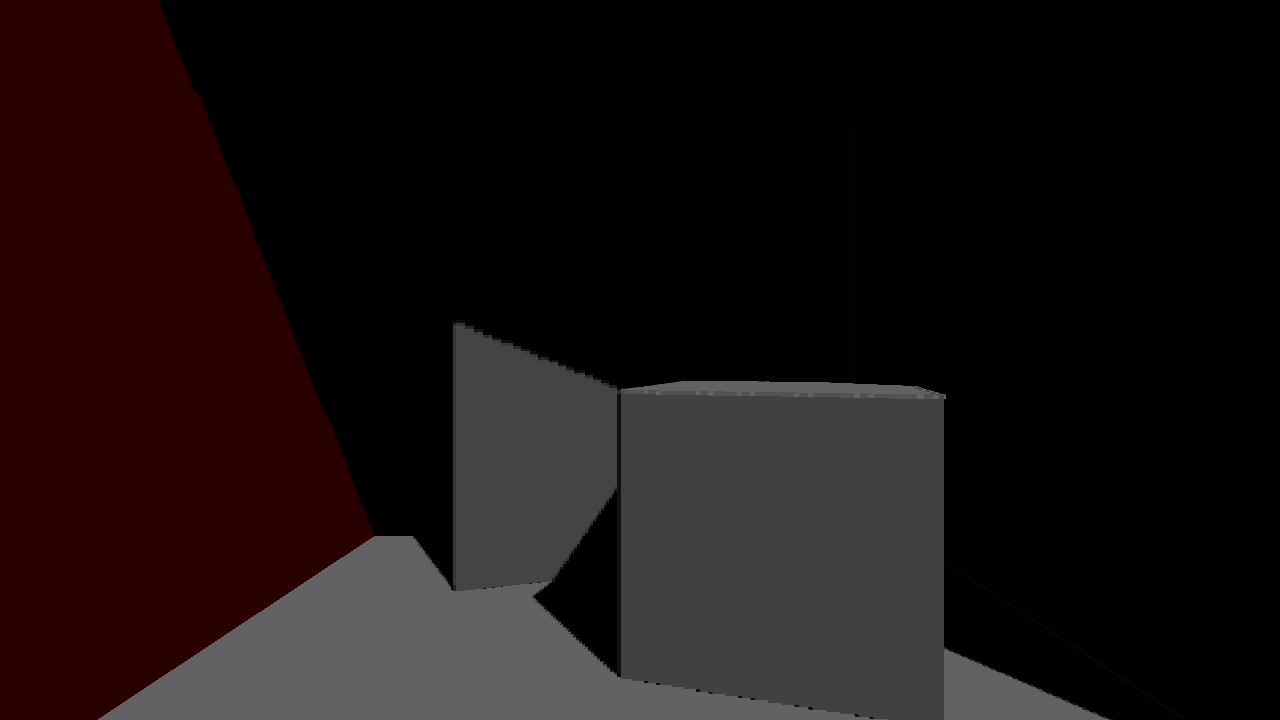
\includegraphics[width=\linewidth]{media/c_voxel_direct.png}
	\end{subfigure}%
	\hspace{0.05\textwidth}
	\begin{subfigure}[t]{0.35\textwidth}
		\centering
		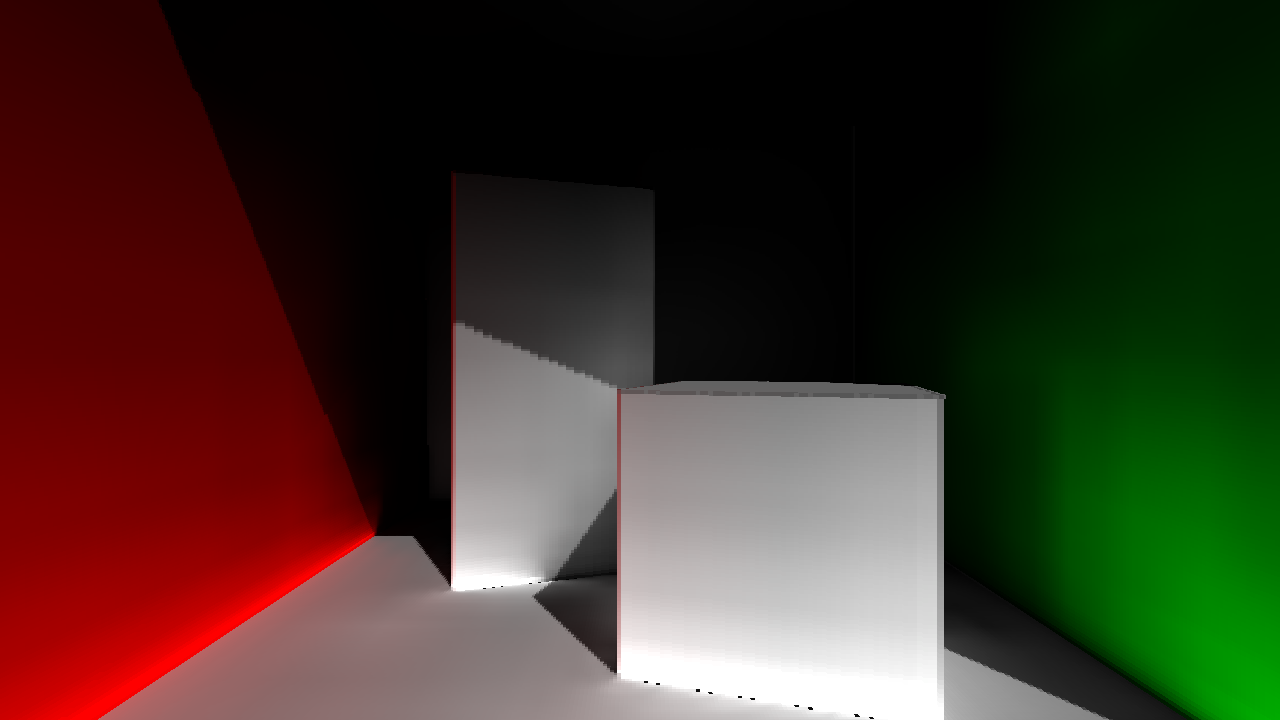
\includegraphics[width=\linewidth]{media/c_voxel_gi.png}
	\end{subfigure}%
	\caption{Resultado de vóxeles con solo iluminación directa y con iluminación global difusa.}
	\label{fig:vgi_scenes}
\end{figure}
% section iluminacion_global_de_voxeles (end)
